\documentclass[12pt]{scrartcl}

\usepackage{indentfirst}
\usepackage{hyperref}

\usepackage{enumitem}
\usepackage{graphicx}
\graphicspath{{Image/}}
\usepackage[a4paper, margin=1in]{geometry}

\title{Advanced Software Lab}
\subtitle{It is an assignment on Latex}
\author{Name: Deep Dey\\Roll: 03}
\date{}
\begin{document}
	\maketitle
	\pagebreak
	\tableofcontents
	\pagebreak
	\listoffigures
	\pagebreak
	\listoftables
	\pagebreak
	
\section*{Abstruct}
	\addcontentsline{toc}{section}{Abstruct}
	Speech under face cover is a new aspect which is faced frequently by forensic
speech experts. Face cover is used by people when they strive to hide their identity.
Face covers not only blocks the scope of Face Recognition but also has huge effect on
speaker recognition by the speech. Different types of face cover and different material
absorbs speech energy differently resulting modulate speech of different kind. This
leads to huge disadvantage in speaker recognition. Again there has been very little
research work done, searching the effects in acoustics of speech through different
face cover. Here is a survey on experiments done in Speaker Recognition under
different Face Cover.	

\pagebreak
	
\section{Introduction}
Speech is foremost way of communication for human being. Speech not only is the
way of communication but also very important to identify a person and get to know about their mental state.\cite{lutz2001programming}\cite{pedregosa2011scikit}\cite{rossum1995python} Some experts can also find physical attributes of a person by
his/her voice. So speech plays a vital role in human life and society.\\

As speech can be used as identifier of a person it is vastly used in different
application as a Biometric security procedure. Since 1990’s speaker recognition gained
huge attraction and many research works have been performed. Now speaker
recognition through Text Dependent (e.g. via password) or Text Independent (via
acoustic qualities) system is more or less available. Forensic speech recognition uses automated system to identify the speaker along with expert listener.\\

But Speaker Recognition under the influence of face cover is a new aspect with
increasing popularity since 2014.

\section{Procedures for Speaker Recognition}
Speaker recognition is broadly classified into two fields. Speaker Verification and
Speaker Identification.
\begin{figure}[h]
	\centering
	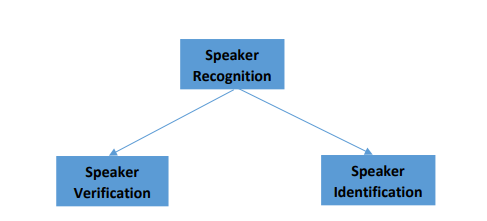
\includegraphics[scale=1]{1.png}
	\caption{Beautiful Picture of Water Body}
	%\label{one}
\end{figure}\\

\pagebreak

\indent Speaker Verification: When a person claims to be someone known to system
and the truth is verified. It is simple in Searching form database. It is just 1:1 mapping
of user given data and database.
\begin{figure}[h]
	\centering
	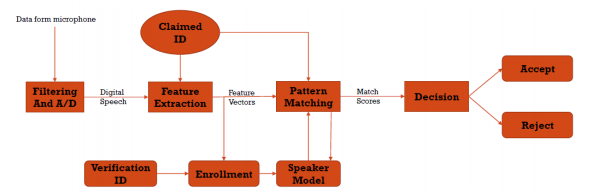
\includegraphics[scale=1]{2.png}
	\caption{ Flowchart for speaker verification [2]}
	%\label{two}
\end{figure}\\
\indent Speaker Identification: When for some unknown person entire database is
searched to find possible match. Here 1:N mapping is held between user data and
database search.
\begin{figure}[h]
	\centering
	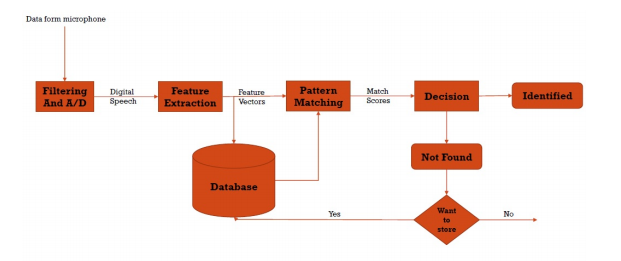
\includegraphics[scale=1]{3.png}
	\caption{  Flowchart of Speaker Identification [2]}
	%\label{three}
\end{figure}\\

\pagebreak

\section{Speaker Recognition form Speech under Face Cover}
Human being is capable of identifying a person by his/her speech (i.e. voice
quality). It is possible for us to recognize some person by their voice even though voice
is molded via some materials which covers the face like Helmet, Mask and Scarf etc.
But in the new area like voice recognition in Computer Science it is a very big
challenge. Intentional voice modulation, in the field of forensic speech analysis, plays a
vital role misleading automated voice recognition system or even expert listener.
Voice modulation can be done by Imitation, speaking under face cover and
synthesized speech.\\

Speech under face cover got the attention after the case of James Foley in Iraq [3].
The modification caused by face cover is generally of two types. <i> Intrinsic (effected
speech due to face cover) and <ii> Extrinsic (signal absorption). The amount of face
covered, degree of contact, restriction in jaw movement and type of the material are
major factors in speech under face cover.
\subsection{Related Works}
In June, 2015 Rahim Saeidi et al. has done a remarkable job in detecting the
speaker under influence of face cover [1]. They studied the change in acoustic due to
face cover with following result,
\begin{figure}[h]
	\centering
	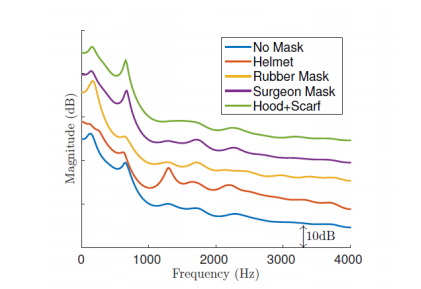
\includegraphics[scale=1]{4.png}
	\caption{[1] Long Term Average Spectrum of a male speaker
 			under the influence of face covering elements}
 	\label{four}
\end{figure}

\pagebreak

They trained a gender dependent Universal Background Model [] with 2048
samples. The results they got are summarized in the following table,

\begin{table}[h]
	\label{Table-1}
	\centering
	\begin{tabular}{ | c | c c c c c | }
		\hline
			Face Cover & No Cover & Helmet & Rubber Mask & Surgeon Mask & Hood+Scarf \\
		\hline
			No Cover & \textbf{95.2} & 94.9 & 88.6 & 94.2 & 93.3\\
			Helmet & 88.5 & \textbf{97.7} & 86.0 & 88.8 & 88.4\\
			Rubber Mask & 90.3 & 96.5 & \textbf{97.1} & 94.1 & 91.4\\
			Surgeon Mask & 95.1 & 96.7 & 90.1 & \textbf{97.9} & 95.6\\
			Hood+Scarf & 90.3 & 85.7 & 82.5 & 94.9 & \textbf{97.0}\\
		\hline
			Number of Tests & 793 & 574 & 543 & 626 & 568\\	
		\hline											
	\end{tabular}
	\caption{[1] Closed-Set Correct Speaker Identification rate in \%}
\end{table}	

\begin{table}[h]
	\label{Table-1}
	\centering
	\begin{tabular}{ | c | c c c c c | }
		\hline
			Face Cover & No Cover & Helmet & Rubber Mask & Surgeon Mask & Hood+Scarf \\
		\hline
			No Cover & 73.9 & 28.7 & 16.9 & 40.7 & 24.5\\
			Helmet & 6.3 & 44.4 & 10.9 & \textbf{9.9} & \textbf{4.6}\\
			Rubber Mask & 4.5 & 12.5 & 56.2 & \textbf{7.2} & \textbf{5.8}\\
			Surgeon Mask & 4.7 & \textbf{6.3} & \textbf{2.8} & 17.1 & 10.4\\
			Hood+Scarf & 10.6 & \textbf{8.0} & \textbf{13.3} & 25.1 & 54.8\\
		\hline
	\end{tabular}
	\caption{ [1] Confusion Matrix for Closed-Set masked identification in \%}
\end{table}

\pagebreak

\section{Conclusion}
Speaker recognition is promising research area with lots of improvements to be
done. It can be used as authentication key, again identification of a person is another
issue.\\

Covering face is an event that frequently occurs in crime cases. For recent events
like Iran [3] and similar incidents it is very important to discover speaker recognition
from speech under face cover.\\

As it shows some limitations in the discussed works it will be noble to use different
artificial intelligence base sophisticated techniques.

\section{Proposed Advancement}
Inspecting the results of the work by Rahim Saeidi et al. a remarkable success rate
for identification is found. But this results shows some limitations

\begin{enumerate}[label=(\roman*)]
	\item Matching in no cover scenario is inferior
	\item The training was done in a small variant of 8 speaker and 5 different frequencies
	\item The samples for matching were taken in suitable environment
\end{enumerate}

So there is a lot of area left for improvement as
\begin{enumerate}[label=(\roman*)]
	\item Improve matching for no-cover scenario;
	\item Improve matching of no-cover with different face cover;
	\item Train with large number of speaker;
	\item Use more face covers for different frequencies;
	\item This may lead to accent and language identification with face cover.
\end{enumerate}

\pagebreak

\bibliographystyle{plain}
\bibliography{ref.bib}
\addcontentsline{toc}{section}{References}

\end{document}